\documentclass[aspectratio=43,x11names]{beamer}
\usetheme{Pittsburgh}
\usepackage{xcolor}
\usepackage[utf8]{inputenc}
\usepackage[german]{babel}
\usepackage{amsmath}
\usepackage{amsfonts}
\usepackage{amssymb}
\usepackage{graphicx}
\usepackage{multicol}
\usepackage{wrapfig}
\usepackage{hyperref}
\usepackage{media9}
\usepackage{tikz}
\usetikzlibrary{shapes,arrows,chains}

\author{Jonas Betzendahl}
\title{Machine Learning Science Slam}

\beamertemplatenavigationsymbolsempty 

%src: https://tex.stackexchange.com/questions/34921/how-to-overlap-images-in-a-beamer-slide
\def\Put(#1,#2)#3{\leavevmode\makebox(0,0){\put(#1,#2){#3}}}

\begin{document}

%------------------------------------------------------------------------------------
\section{Introduction}

\begin{frame}
\begin{center}
\vfill
\huge BOT or NOT?
\normalsize 
\smallskip
\smallskip

Das was, weshalb und wie des Maschinellen Lernens 
\bigskip\bigskip

\large Jonas Betzendahl, M.Sc.
\bigskip\bigskip

\href{https://twitter.com/lambdatotoro}{
\includegraphics[scale=0.125]{images/twitter_logo.png}}
\href{https://chaos.social/@lambdatotoro}{\includegraphics[scale=0.125]{images/mastodon_logo.png}}
\href{https://github.com/jbetzend}{
\includegraphics[scale=0.125]{images/github_logo.png}}
\href{https://whispeer.de/en/user/jbetzend}{
\includegraphics[scale=0.125]{images/whispeer_logo.png}}

\texttt{@lambdaTotoro (@chaos.social)}
\end{center}
\end{frame}

%------------------------------------------------------------------------------------

\begin{frame}
\frametitle{Small Talk in Intelligent Systems}

\begin{multicols}{2}

Mein Studium:\\ \glqq Intelligente Systeme\grqq .
\medskip

Was war wohl die häufigste Frage an meinen Studiengang?

\pause

\begin{center}
\glqq Na, wie lange dauert\\ es noch bis zur\\ Roboterapokalypse?\grqq
\end{center}

\columnbreak

\begin{center}

\includegraphics[height=0.7\textheight,keepaspectratio]{images/mtt.png} 
\end{center}
\end{multicols}
\end{frame}

\begin{frame}
\begin{center}

\includegraphics[width=\textwidth]{images/amazon-logo.jpg} 
\end{center}
\end{frame}

\begin{frame}
\begin{center}

\includegraphics[width=\textwidth]{images/amazon-one-wallet.jpg} 
\end{center}
\end{frame}

\begin{frame}
\begin{center}
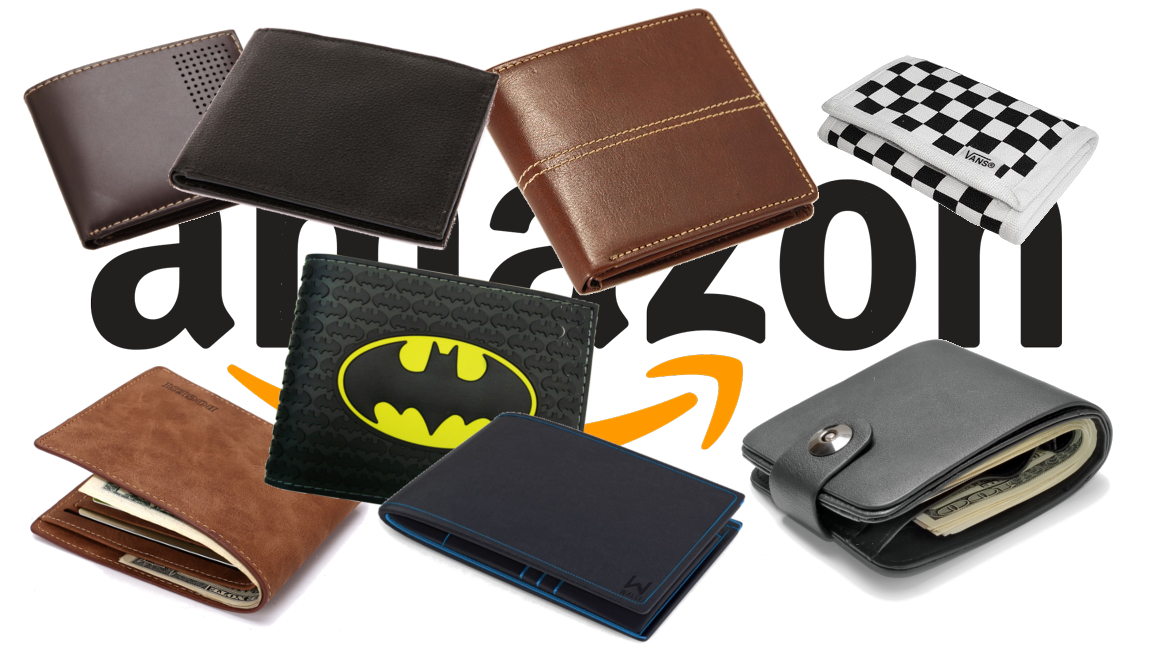
\includegraphics[width=\textwidth]{images/amazon-buncha-wallets.jpg} 
\end{center}
\end{frame}

%------------------------------------------------------------------------------------

\section{Warum Maschinelles Lernen?}

\begin{frame}
\begin{center}
\huge
Warum überhaupt\\Maschinelles Lernen?
\end{center}
\end{frame}

%------------------------------------------------------------------------------------

\begin{frame}
\begin{center}
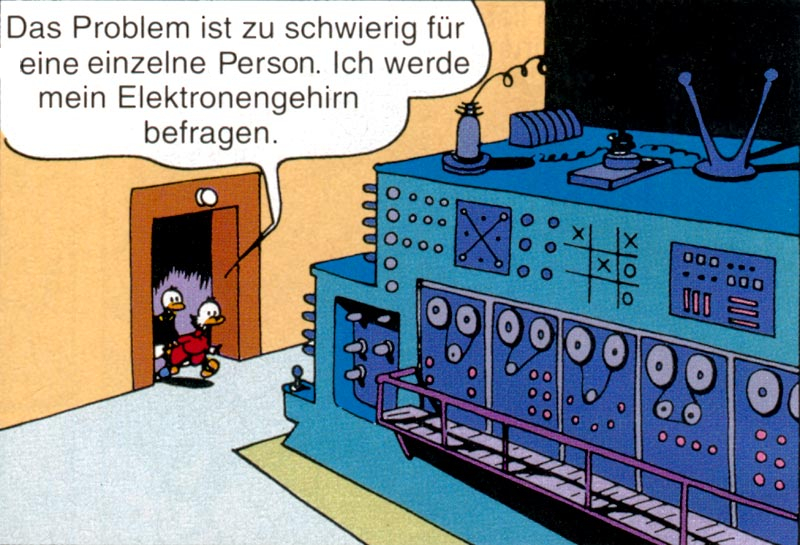
\includegraphics[width=\textwidth]{images/elektronengehirn} 
\end{center}
\end{frame}

\begin{frame}
\begin{center}
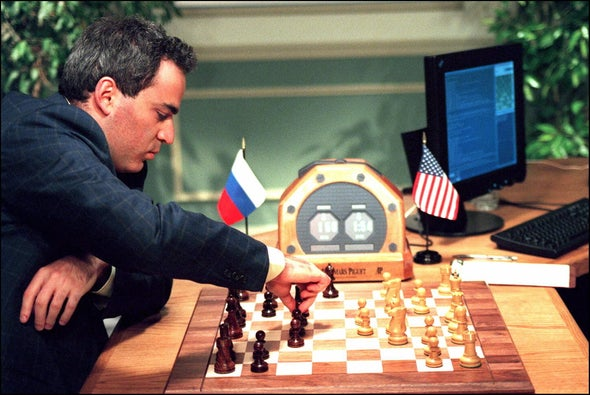
\includegraphics[width=\textwidth]{images/kasparov} 
\end{center}
\end{frame}

\begin{frame}
\frametitle{Verschiedene Welten (1)}

\begin{center}

% Klassisches Programmieren
\begin{tikzpicture}[scale=1.15]
\node[draw, rounded corners, text centered, minimum height=4.5em, text width=8em] at (0,0) (prog) {Klassisches \\ Programmieren};

\node[] at (-3.5,-0.4) (d1) {Daten};
\node[] at (-3.5,0.4) (r1) {Regeln};
\node[] at (3.5,-0) (a1) {Antworten};

\draw[->, very thick] (prog) -- (a1);
\draw[->, very thick, shorten >=3pt] (d1) -- (d1-|prog.west);
\draw[->, very thick, shorten >=3pt] (r1) -- (r1-|prog.west);

\node[draw, rounded corners, text centered, minimum height=4.5em, text width=8em] at (0,-3) (ml) {Maschinelles \\ Lernen};

\node[] at (-3.5,-3.4) (d2) {Daten};
\node[] at (-3.5,-2.6) (a2) {Antworten};
\node[] at (3.5,-3) (r2) {Regeln};

\draw[->, very thick] (ml) -- (r2);
\draw[->, very thick, shorten >=3pt] (d2) -- (d2-|ml.west);
\draw[->, very thick, shorten >=3pt] (a2) -- (a2-|ml.west);
\end{tikzpicture}

\end{center}
\end{frame}

\begin{frame}[fragile]
\frametitle{Verschiedene Welten (2)}

\begin{minipage}{0.45\textwidth}
\begin{center}
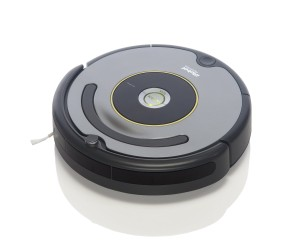
\includegraphics[width=\textwidth]{images/roomba} 
\end{center}
\end{minipage}
\begin{minipage}{0.45\textwidth}
\begin{center}
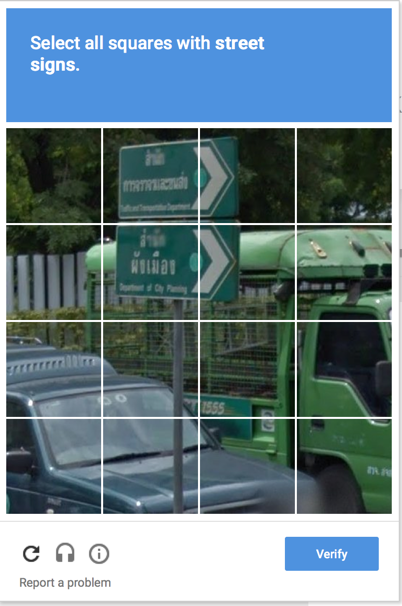
\includegraphics[width=0.75\textwidth]{images/recaptcha}
\end{center}
\end{minipage}

\end{frame}

%------------------------------------------------------------------------------------

\section{Wie funktioniert Maschinelles Lernen?}

\begin{frame}
\begin{center}
\huge
Wie funktioniert\\Maschinelles Lernen?
\end{center}
\end{frame}

\begin{frame}
\begin{center}
\Large Imitation - Mehr als nur Anerkennung!
\medskip\medskip

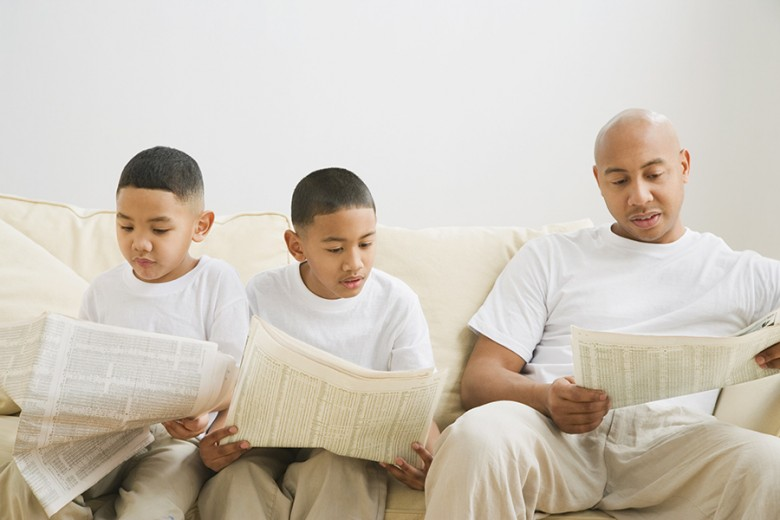
\includegraphics[scale=0.35]{images/imitation}
\end{center}
\end{frame}

\begin{frame}
\begin{center}
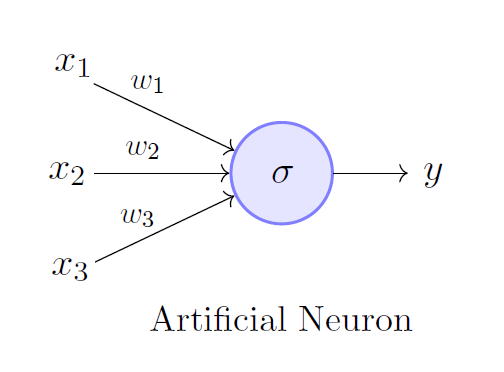
\includegraphics[width=\textwidth]{images/perceptron} 
\end{center}
\end{frame}

\begin{frame}
\begin{center}
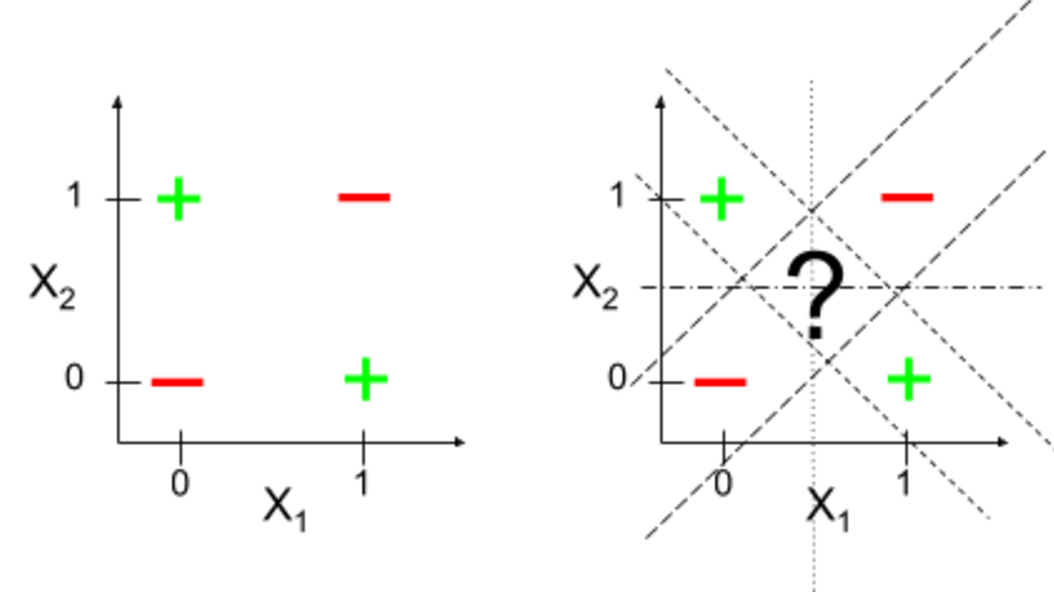
\includegraphics[width=\textwidth]{images/xor} 
\end{center}
\end{frame}

\begin{frame}
\begin{center}
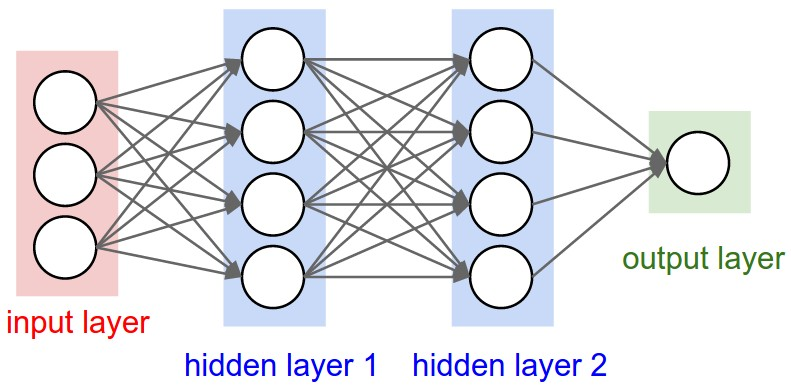
\includegraphics[width=\textwidth]{images/simple_neural_network_header.jpg} 
\end{center}
\end{frame}

\begin{frame}
\begin{center}
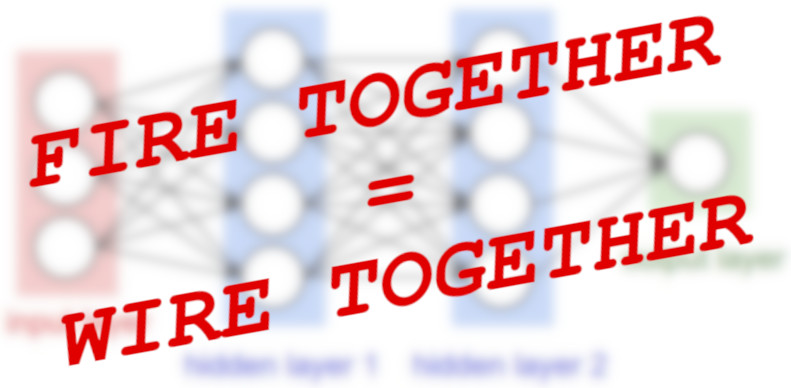
\includegraphics[width=\textwidth]{images/simple_neural_network_header_FW.jpg} 
\end{center}
\end{frame}

\begin{frame}
\frametitle{Was ist einfach?}

\begin{minipage}{0.45\textwidth}
Generell gilt: Je \dots
\bigskip

\begin{itemize}
\item übersichtlicher
\item mehr Daten
\item weniger Rückfragen
\end{itemize}
\bigskip

\dots desto gut! Aber es gibt ein paar beliebte Fallen!

\end{minipage}
\begin{minipage}{0.45\textwidth}
\begin{center}

\includegraphics[width=0.95\textwidth]{images/learning} 
\end{center}
\end{minipage}

\end{frame}

\begin{frame}
\frametitle{Nichts ist wie es scheint!}
\begin{center}
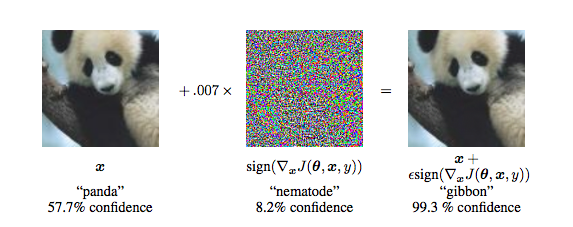
\includegraphics[width=\textwidth,keepaspectratio]{images/recog_panda.png} 
\end{center}
\end{frame}

\begin{frame}
\frametitle{Nichts ist wie es scheint!}
\begin{center}
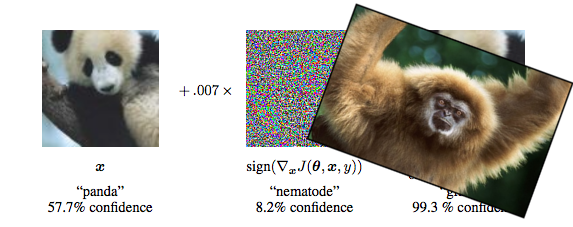
\includegraphics[width=\textwidth, keepaspectratio]{images/recog_gibbon.png} 
\end{center}
\end{frame}

\begin{frame}
\frametitle{Was wird gelernt?}
\begin{center}
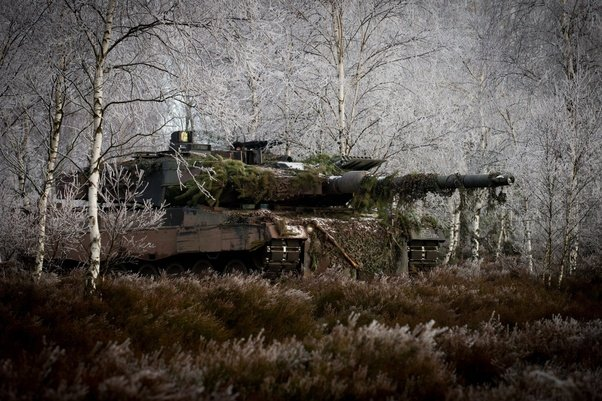
\includegraphics[width=0.85\textwidth]{images/tank} 
\end{center}
\end{frame}

%------------------------------------------------------------------------------------

\section{Word2Vec}

\begin{frame}
\begin{center}
\huge
\emph{Bot or Not?}
\bigskip

\Large
Wie kommen wir\\ vom Lernen zum Gedicht?
\end{center}
\end{frame}

\begin{frame}
\frametitle{word2vec}
\begin{center}
``You shall know a word by the company it keeps''\\
\qquad\qquad\qquad\qquad -- J.R. Firth
\bigskip\bigskip

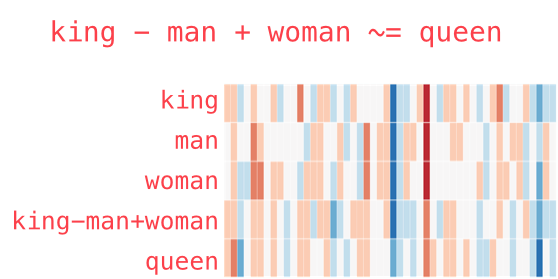
\includegraphics[width=0.8\textwidth]{images/word2vec} 
\end{center}
\end{frame}

\begin{frame}
\frametitle{word2vec + Tensorflow = ???}
\begin{center}

\includegraphics[width=0.95\textwidth]{images/funnel} 
\end{center}
\end{frame}

%------------------------------------------------------------------------------------

\begin{frame}[fragile]
\frametitle{Computerkunst}

\begin{minipage}{0.45\textwidth}
\begin{center}
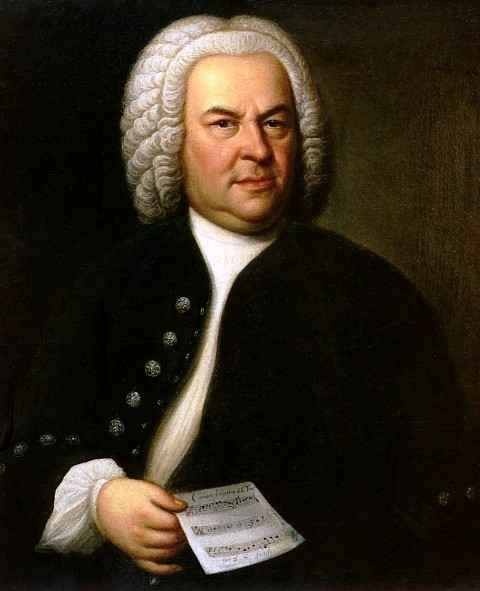
\includegraphics[width=\textwidth, keepaspectratio]{images/bach} 
\end{center}
\end{minipage}
\begin{minipage}{0.45\textwidth}
\begin{center}
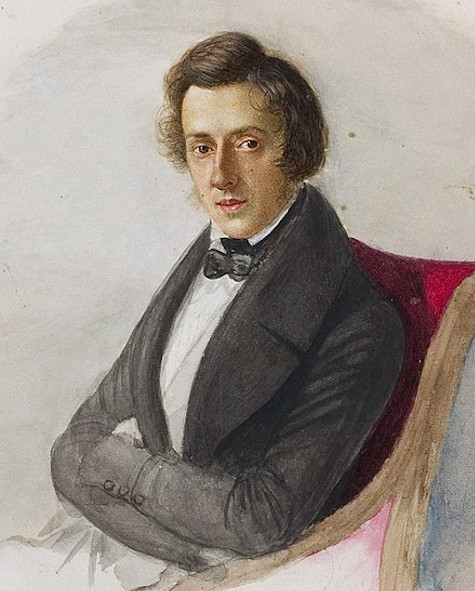
\includegraphics[width=\textwidth, keepaspectratio]{images/chopin} 
\end{center}
\end{minipage}
\end{frame}

%------------------------------------------------------------------------------------


\begin{frame}[fragile]
\begin{multicols}{2}

\vspace*{73pt}

\includegraphics[scale=0.6]{images/Happy-Thumbs-Up-Robot.png} 

\columnbreak

\vspace*{40pt}

\Huge
\hspace*{-30pt}Vielen Dank\\ für's\\ Zuhören!
\end{multicols}
\end{frame}

\end{document}

